\documentclass[standalone, version=1.0]{huangfusl-template}
\usepackage{tikz}
\begin{document}
    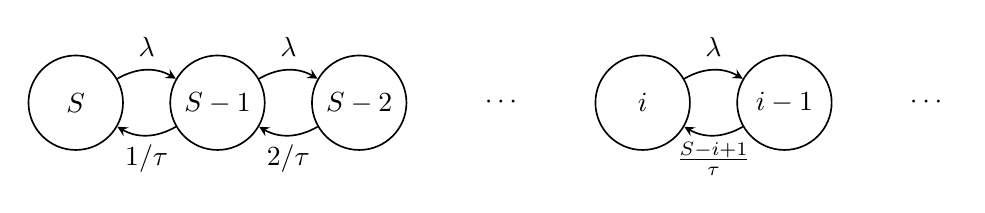
\begin{tikzpicture}
        [
            Node/.style={circle, draw=black, minimum size=12mm, semithick},
            EmptyNode/.style={circle, draw=white},
            Connection/.style={semithick, -stealth, draw=black}
        ]
        \node[Node] (S) at (0, 0) {$S$};
        \node[Node, right of=S, xshift=0.8cm] (S-1) {$S-1$};
        \node[Node, right of=S-1, xshift=0.8cm] (S-2) {$S-2$};
        \node[EmptyNode, right of=S-2, xshift=0.8cm] (gap1) {$\cdots$};
        \node[Node, right of=gap1, xshift=0.8cm] (i) {$i$};
        \node[Node, right of=i, xshift=0.8cm] (i-1) {$i-1$};
        \node[EmptyNode, right of=i-1, xshift=0.8cm] (gap2) {$\cdots$};

        \path[Connection] (S) to[bend left=30] node[yshift=0.3cm] {$\lambda$} (S-1);
        \path[Connection] (S-1) to[bend left=30] node[yshift=0.3cm] {$\lambda$} (S-2);
        \path[Connection] (i) to[bend left=30] node[yshift=0.3cm] {$\lambda$} (i-1);

        \path[Connection] (S-1) to[bend left=30] node[yshift=-0.3cm] {$1 / \tau$} (S);
        \path[Connection] (S-2) to[bend left=30] node[yshift=-0.3cm] {$2 / \tau$} (S-1);
        \path[Connection] (i-1) to[bend left=30] node[yshift=-0.3cm] {$\frac{S - i + 1}{\tau}$} (i);
    \end{tikzpicture}
\end{document}